% \special{dvipdfmx:config z 0} % disable pdf compress to boost compilation time, comment this out for release
\documentclass{article}

\usepackage{amsmath, amsfonts, amsthm, amssymb} 
\usepackage{listings}
\usepackage{graphicx}
\usepackage{float}
\usepackage{subfigure}
\usepackage{geometry}
\usepackage{hyperref}
\usepackage[parfill]{parskip} % no newline indent
\usepackage{enumitem} % enumerate / ordered list
\usepackage{booktabs} % three-line table
\usepackage{array}   % for \newcolumntype macro
\usepackage{listings} % MATLAB code block
\usepackage{pdfpages} % include external pdf pages
\usepackage[bottom]{footmisc} % move footnote to the bottom
\newcolumntype{C}{>{$}c<{$}} % math-mode version of "l" column type

\theoremstyle{definition} % definition
\newtheorem{definition}{Definition}[section]
\newtheorem{theorem}{Theorem}[section]
\newtheorem{remark}{Remark}[section]

\newcommand{\dd}{\mathrm{d}}
\newcommand{\RR}{\mathbb{R}}
\newcommand{\NN}{\mathbb{N}}
\newcommand{\ZZ}{\mathbb{Z}}
\newcommand{\CC}{\mathbb{C}}
\newcommand{\PP}{\mathbb{P}}


\lstset{
  language=Matlab, 
  frame=shadowbox, 
  numbers=left,
  breaklines=true
}

\geometry{
	paper=a4paper, 
	top=2.5cm,
	bottom=2.5cm, 
	left=2.5cm, 
	right=3cm,
	headsep=0.75cm, 
}
\title{ROB 422 HW 5}
\author{Yulun Zhuang \\ \href{mailto:yulunz@umich.edu}{yulunz@umich.edu}}
\date{\today}

\begin{document}

\maketitle

\section*{Questions}
\subsection*{Derive $P(\neg a) = 1-P(a)$}
\begin{proof}
    \begin{align*}
        1 &= P(a\lor \neg a)\\
        &= P(a) + P(\neg a) - P(a\land \neg a)\\
        &= P(a) + P(\neg a) \Leftarrow P(a\land \neg a) = 0\\
        \Rightarrow P(\neg a) &= 1-P(a)
    \end{align*}
\end{proof}

\subsection*{AI Book, Chapter 13, Ex. 13.8}
\begin{enumerate}[label=\alph*.]
    \item $P(toothache) = 0.108 + 0.012 + 0.016 + 0.064 = 0.2$
    \item $P(Cavity) = <0.2, 0.8>$
    \item $P(Toothache | cavity) = <0.6, 0.4>$
    \item $P(Cavity | toothache \lor catch) = <0.4615, 0.5384>$
\end{enumerate}

\subsection*{AI Book, Chapter 13, Ex. 13.16}

\begin{enumerate}[label=\alph*.]
    \item 
    \begin{proof}
        \begin{align*}
            P(X|Y, e) P(Y|e) &= \frac{P(X, Y, e)}{P(Y, e)} \frac{P(Y, e)}{P(e)} \\
            &= \frac{P(X, Y, e)}{P(e)} \\
            &= P(X, Y | e)
        \end{align*}
    \end{proof}
    \item 
    \begin{proof}
        \begin{align*}
            \frac{P(X|Y, e)P(Y | e)}{P(X|e)} &= \frac{P(X, Y | e)}{P(X|e)}\\
            &= P(Y|X,e)
        \end{align*}
    \end{proof}
\end{enumerate}

\subsection*{AI Book, Chapter 14, Ex. 14.5 part a}
Let $X$ be the set of all variables in the Bayesian Network except for $Y$ and $MB(Y )$.
Given $MB(Y)$, we have $P(X|Y,mb(Y)) = P(X|mb(Y)) = \alpha P(X,mb(Y))$. 
Also parents of $Y$ ’s children are a subset of ${Y }\cup MB(Y)$, without including any variables in $X$.
Thus, all the CPT entries for $Y$ ’s children including the expand of $P(X,mb(Y))$, are constants and can be subsumed in $\alpha$.

% \subsection*{AI Book, Chapter 14, Ex. 14.6}
% TODO

\subsection*{AI Book, Chapter 15, Ex. 15.2}
\begin{enumerate}[label=\alph*.]
    \item $\forall t$, we have $\mathbf{P}(R_t | u_{1: t})=\alpha \mathbf{P}(u_t | R_t) \sum_{R_{t-1}} \mathbf{P}(R_t | R_{t-1}) P(R_{t-1} | u_{1: t-1})$ which increases monotonically.\\
    For the fixed point, let its probabilities be $<\rho, 1-\rho>$, plug in $\mathbf{P}(R_t | u_{1: t})=\mathbf{P}(R_{t-1} | u_{1: t-1})$ and we have $\langle\rho, 1-\rho\rangle=\alpha\langle 0.9,0.2\rangle\langle 0.7,0.3\rangle \rho+\langle 0.3,0.7\rangle(1-\rho)$. Solving it we find $\rho \approx 0.8933$.
    \item % TODO
    \begin{align*}
        \mathbf{P}(R_{2+k} | U_1, U_2) & =\langle 0.7,0.3\rangle P(r_{2+k-1} | U_1, U_2)+\langle 0.3,0.7\rangle P(\neg r_{2+k-1} | U_1, U_2) \\
        \mathbf{P}(r_{2+k} | U_1, U_2) & =0.7 P(r_{2+k-1} | U_1, U_2)+0.3(1-P(r_{2+k-1} | U_1, U_2)) \\
        & =0.4 P(r_{2+k-1} | U_1, U_2)+0.3\\
        \Rightarrow P(r{2+k}|U_1, U_2) &= 0.5
    \end{align*}
\end{enumerate}

\subsection*{AI Book, Chapter 15, Ex. 15.13}
Let $S_t$ denotes whether a student gets enough sleep, $R_t$ denotes whether a student has red eyes in class, and $C_t$ denotes whether a student sleeps in class. $S_t$ is a parent of $S_{t+1}$, $R_t$ and $C_t$.

Given
\begin{align*}
        P(s_0) & =0.7 \\
        P(s_{t+1} | s_t) & =0.8 \\
        P(s_{t+1} | \neg s_t) & =0.3 \\
        P(r_t | s_t) & =0.2 \\
        P(r_t | \neg s_t) & =0.7 \\
        P(c_t | s_t) & =0.1 \\
        P(c_t | \neg s_t) & =0.3
\end{align*}

To reformulate it as a hidden Markov model, define a new variable $O_t$ that represent the daily observation from the professor, combining the information about red eyes and sleeping in class.

\[
    O_t = 
    \begin{cases} 
    1 & \text{if } \neg R_t \text{ and } \neg C_t \\
    2 & \text{if } R_t \text{ and } \neg C_t \\
    3 & \text{if } \neg R_t \text{ and } C_t \\
    4 & \text{if } R_t \text{ and } C_t
    \end{cases}
\]

The probability tables for this HMM are:

1. Initial state probabilities:
\begin{align*}
   P(s_0) & = 0.7
\end{align*}

2. Transition probabilities:
\begin{align*}
   P(s_{t+1} | s_t) & = 0.8 \\
   P(s_{t+1} | \neg s_t) & = 0.3
\end{align*}

3. Emission probabilities:
\begin{align*}
    P(o_t = 1 | s_t) & = P(\neg r_t | s_t) P(\neg c_t | s_t) = 0.56\\
    P(o_t = 2 | s_t) & = P(r_t | s_t) P(\neg c_t | s_t) = 0.14 \\
    P(o_t = 3 | s_t) & = P(\neg r_t | s_t) P(c_t | s_t) = 0.24\\
    P(o_t = 4 | s_t) & = P(r_t | s_t) P(c_t | s_t) = 0.06
\end{align*}


\subsection*{PF vs. EKF vs. UKF}

\begin{enumerate}[label=\alph*.]
    \item \textbf{Particle Filter}: High computational cost when simulating large amount of particles, can handle highly non-linear dynamics with multi-model state distributions.
    \item \textbf{Extended Kalman Filter}: Polynomial computational cost in state and measurement dimensionalities, can handle non-linear dynamics using first order local linear approximation, but can diverge if too large non-linearity, can handle only single-model state distributions.
    \item \textbf{Unscented Kalman Filter}: Same computational complexity as EKF, can handle single-model distributed states with non-linear dynamics using second order Taylor approximation.
\end{enumerate}


\section*{Implementation}

\subsection*{Kalman Filter}

\subsubsection*{a. System derivations}
Define the state $\mathbf{x} = [x, y]^T$, the input $\mathbf{u} = [u_1, u_2]^T$. The system models can be derived as following.
\begin{align*}
    \mathbf{x}_{t+1} &= 
    \underbrace{
    \begin{bmatrix}
        1 & 0 \\ 0 & 1
    \end{bmatrix}
    }_A
    \mathbf{x}_t + 
    \underbrace{
    \begin{bmatrix}
        1.5 & 0.1 \\ 0.2 & -0.5
    \end{bmatrix}
    }_B
    \mathbf{u} + 
    \begin{bmatrix}
        \zeta_x &\\&\zeta_y 
    \end{bmatrix}
    \\
    \mathbf{z} &= 
    \underbrace{
    \begin{bmatrix}
        1.05 & 0.01 \\ 0.01 & 0.9
    \end{bmatrix}}
    _C
    \mathbf{x} + 
    \begin{bmatrix}
        \delta_1 &\\&\delta_2
    \end{bmatrix}
\end{align*}


\subsubsection*{b. Noise covariance estimation}
The motion noise covariance $R$ and the sensor noise covariance $Q$ are estimated as following.

\begin{align*}
    R = 
    \begin{bmatrix}
        2.5069e^{-3} & 1.7995e^{-5}\\
        1.7995e^{-5} & 2.5106e^{-3}
    \end{bmatrix}\\
    Q = 
    \begin{bmatrix}
        4.8695e^{-2} & 5.8636e^{-3}\\
        5.8636e^{-3} & 1.0121e^{-0}
    \end{bmatrix}
\end{align*}

\subsubsection*{c. KF execution}
The total errors (sum of the norm of state difference for each frame) are $21.8194$.

\begin{figure}[H]
    \centering
        \textsf{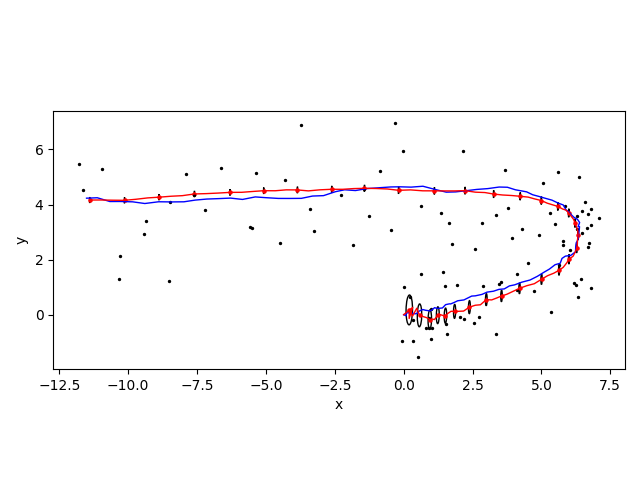
\includegraphics[width=0.9\columnwidth]{kf.png}}
        \caption{The comparison of estimated (in red) and ground truth (in blue) trajectories. The black dots shows the original measurements while black ellipses are the estimated pose covariance.}
        \label{fig:kf}
\end{figure}


\end{document}